\documentclass{article}
\usepackage{graphicx}
\usepackage[margin=1in]{geometry}
%\usepackage{amsmath}

\begin{document}
\title{16-831 Project 3: Robot Localization}
\author{Alex Brinkman, Shivam Gautam, Tushar Agrawal}
\maketitle

\begin{figure}[!h]
    \centering
    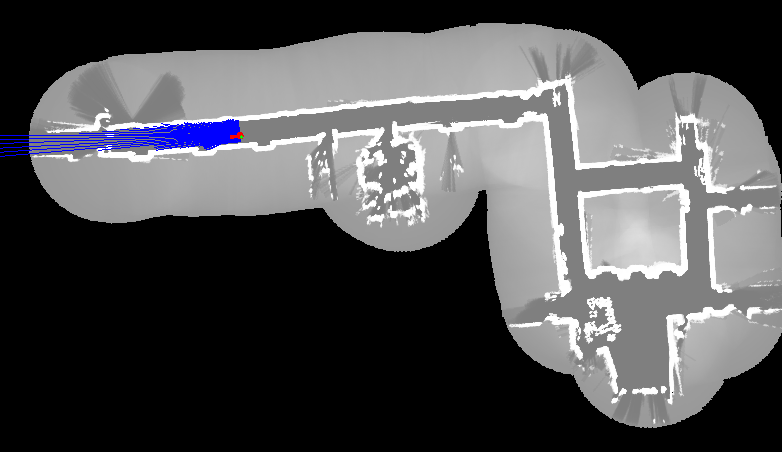
\includegraphics[width=4.0in]{media/graphics_example.png}
    \caption{Visualization of the Particle Filter after Convergence}
\label{fig:1}
\end{figure}

\section{Approach}
	We started by first developing the modules in isolation to facilitate future integration. We started by independently developing the sensor model, motion model, ray tracing, and graphics engine, and log-streaming modules first. We performed unit testing on each to verify they were working properly, relying heavily on the graphics to validate the complex modules. Once the modules were build up, we integrated the modules and debugged the interfacing issues and added importance resampling. Since the modules were tested independently, this was relatively painless. Finally, we refined the pipeline to improve runtime and tuned the particle filter parameters to find a good trade-off between convergence speed and correctness. Figure \ref{fig:1} depicts the final outcome of the particle filter.

\section{Implementation}
	We implemented the particle filter in C++ and used a private git repo in our workflow.  All modules were implemented as stand alone classes and invoked in executable scripts.  The final integration took the individual classes and encapsulated the modules while exposing configuration parameters to ease tuning. We used GNUplot-iostream to visualize 1D data like the sensor model and the SFML library to visualize the map, particles, and laser readings.  

\subsection{Sensor Model}
	The sensor model consists of a superposition of an exponential decay function, Gaussian distribution, uniform distribution, and max value.  The Gaussian distribution mean is placed at the expected range measurement with a tunable variance. Since the we wanted to sum the log-likelihood of each of the 180 range readings, the uniform distribution of the model is 1 so for any range measurement this provides a log-likelihood of at least zero. The decay function plays a small role in the overall shape of the function. The Gaussian was tuned first by using reasonable values for gain factor and standard deviation.  We found that once we set the initial values to something reasonable, we did not have to tune this model much to get the performance we desired. Figure \ref{fig:2} shows the final sensor model used in our tuned model and Figure \ref{fig:3} shows the final parameters.
\begin{figure}[!h]
    \centering
    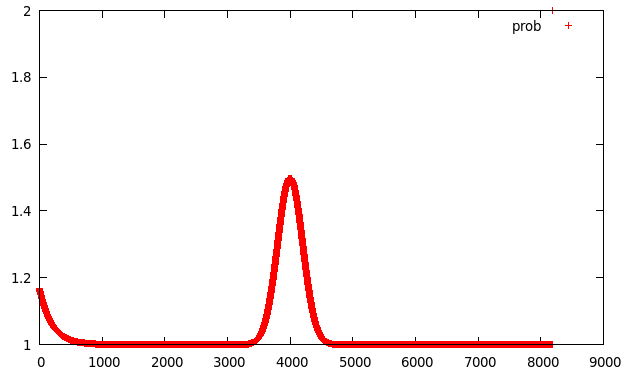
\includegraphics[width=2.5in]{media/sensor_model.png}
    \caption{Sensor Model for reference reading for 4000cm, X-axis is cm}
\label{fig:2}
\end{figure}

\begin{figure}[!h]
    \centering
    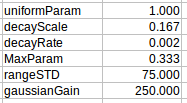
\includegraphics[width=2.0in]{media/sensor_model_parameters.png}
    \caption{Final Sensor Model Parameters}
\label{fig:3}
\end{figure}

\subsection{Motion Model}



\begin{figure}[!h]
    \centering
    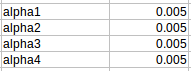
\includegraphics[width=2.0in]{media/motion_model_parameters.png}
    \caption{Final Motion Model Parameters}
\label{fig:4}
\end{figure}

\subsection{Ray Tracing}

\begin{figure}[!h]
    \centering
    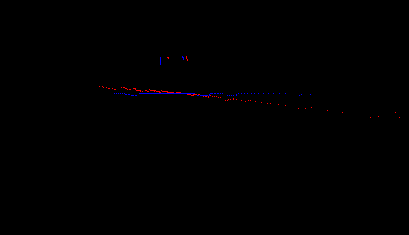
\includegraphics[width=2.5in]{media/ray_tracing.png}
    \caption{Ray Tracing(Red) Validation against Logged Data(Blue)}
\label{fig53}
\end{figure}

\subsection{Importance Resampling}


\section{Results}

\section{Future Work}



\end{document}